\documentclass[12pt, twoside]{article}
\usepackage[letterpaper, margin=1in, headsep=0.5in]{geometry}
\usepackage[english]{babel}
\usepackage[utf8]{inputenc}
\usepackage{amsmath}
\usepackage{amsfonts}
\usepackage{amssymb}
\usepackage{tikz}
\usetikzlibrary{quotes, angles}
\usepackage{graphicx}
\usepackage{enumitem}
\usepackage{multicol}

\newif\ifmeta
\metatrue %print standards and topics tags

\title{Regents Geometry}
\author{Chris Huson}
\date{September 2020}

\usepackage{fancyhdr}
\pagestyle{fancy}
\fancyhf{}
\renewcommand{\headrulewidth}{0pt} % disable the underline of the header
\raggedbottom


\fancyhead[LE]{\thepage}
\fancyhead[RO]{\thepage \\ Name: \hspace{4cm} \,\\}
\fancyhead[LO]{BECA / Dr. Huson / Geometry 09-Congruence-transformations\\* pset ID: 155}

\begin{document}

\subsubsection*{9-4CW-Triangle-congruence-proof}
\begin{enumerate}
\item Given $\triangle ABC$ and $\triangle EFG$ with $\overline{AB} \cong \overline{EF}$, $\overline{BC} \cong \overline{FG}$, and $\overline{AC} \cong \overline{EG}$. \\Prove $\triangle ABC \cong \triangle EFG$ (by filling in the blanks below)\\[0.5cm]
    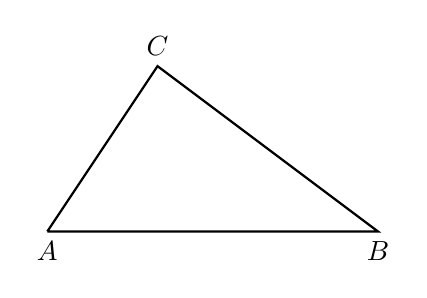
\begin{tikzpicture}[scale=0.7]
        \draw [thick]
          (2,0)node[below]{$A$}--
          (8,0)node[below]{$B$}--
          (4,3)node[above]{$C$} --(2,0);
      \end{tikzpicture}
      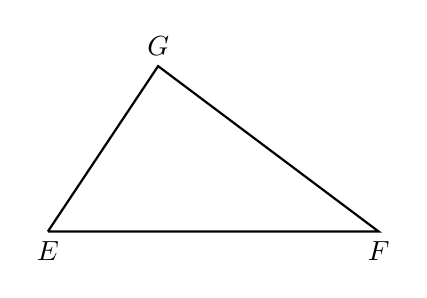
\begin{tikzpicture}[scale=0.7]
        \draw [thick]%(0,0)node[below]{$A$}--
        (2,0)node[below]{$E$}--
        (8,0)node[below]{$F$}--
        (4,3)node[above]{$G$} --(2,0);
    \end{tikzpicture}
    \begin{multicols}{2}
      \underline{Statement} \\
      \underline{Reason}
    \end{multicols}
    \begin{multicols}{2}
      \raggedcolumns
      \begin{enumerate}[label={\arabic*)}]
        \item $\triangle ABC$, $\triangle EFG$
        \item $\overline{AB} \cong \overline{EF}$
        \item $\overline{BC} \cong \overline{FG}$, $\overline{AC} \cong \overline{EG}$
        \item $\triangle ABC \cong \triangle EFG$
      \end{enumerate}
      \begin{enumerate}[label={\arabic*)}]
        \item Given
        \item \rule{4cm}{0.15mm}
        \item \rule{4cm}{0.15mm}
        \item \rule{4cm}{0.15mm}
      \end{enumerate}
    \end{multicols}

\item Two parallel lines intersect a transversal,  $\overleftrightarrow{MD} || \overleftrightarrow{BC}$, $\overline{MD} \cong \overline{BC}$ and $M$ is the midpoint of $\overline{AB}$. Prove $\triangle ADM \cong \triangle MCB$.
   \begin{center}
   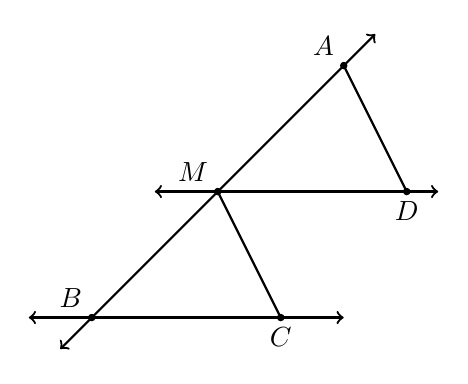
\begin{tikzpicture}[scale=0.8]
     \draw [<->, thick] (-1,0)--(0,0)--(4,0);
     \draw [<->, thick] (-0.5,-0.5)--(4,4)--(4.5,4.5);
     \draw [<->, thick] (1,2)--(5, 2)--(5.5,2);
     \draw [-, thick] (4,4)--(5, 2);
     \draw [-, thick] (2,2)--(3,0);
     \draw [fill] (4,4) circle [radius=0.05] node[above left]{$A$};
     \draw [fill] (5, 2) circle [radius=0.05] node[below]{$D$};
     \draw [fill] (2,2) circle [radius=0.05] node[above left]{$M$};
     \draw [fill] (0,0) circle [radius=0.05] node[above left]{$B$};
     \draw [fill] (3,0) circle [radius=0.05] node[below]{$C$};
   \end{tikzpicture}
   \end{center}
   \begin{multicols}{2}
     \underline{Statement} \\
     \underline{Reason}
   \end{multicols}
   \begin{multicols}{2}
     \raggedcolumns
     \begin{enumerate}[label={\arabic*)}] %\usepackage{enumitem}
       \item $\overleftrightarrow{MD} || \overleftrightarrow{BC}$ \vspace{0.3cm}
       \item $M$ is the midpoint of $\overline{AB}$ \vspace{0.3cm}
       \item \rule{2cm}{0.15mm} $\cong \overline{BC}$ \vspace{0.3cm}
       \item $\angle AMD \cong \angle MBC$ \vspace{0.3cm}
       \item \rule{2cm}{0.15mm} $\cong \overline{AM}$ \vspace{0.3cm}
       \item $\triangle ADM \cong \triangle MCB$  \vspace{0.3cm}
     \end{enumerate}
     \begin{enumerate}[label={\arabic*)}]
       \item \rule{4cm}{0.15mm} \vspace{0.3cm}
       \item \rule{4cm}{0.15mm} \vspace{0.3cm}
       \item Given \vspace{0.3cm}
       \item \rule{4cm}{0.15mm} \vspace{0.3cm}
       \item Definition of a midpoint \vspace{0.3cm}
       \item \rule{4cm}{0.15mm} \vspace{0.3cm}
     \end{enumerate}
   \end{multicols}

\newpage
\item Given $\triangle ABC$ and $\triangle EFG$ with $\angle A \cong \angle E$, $\overline{AB} \cong \overline{EF}$, and $\overline{AC} \cong \overline{EG}$. Prove $\triangle ABC \cong \triangle EFG$.\\[0.5cm]
     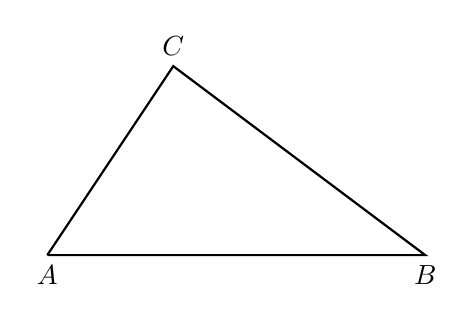
\begin{tikzpicture}[scale=0.8]
         \draw [thick]
           (2,0)node[below]{$A$}--
           (8,0)node[below]{$B$}--
           (4,3)node[above]{$C$} --(2,0);
       \end{tikzpicture}
       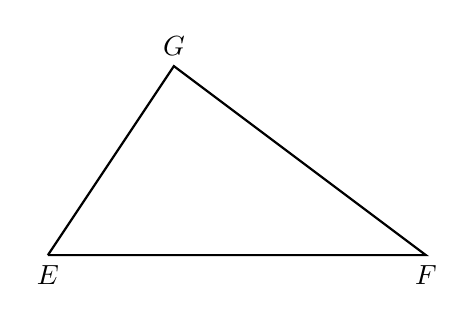
\begin{tikzpicture}[scale=0.8]
         \draw [thick]%(0,0)node[below]{$A$}--
         (2,0)node[below]{$E$}--
         (8,0)node[below]{$F$}--
         (4,3)node[above]{$G$} --(2,0);
     \end{tikzpicture}

     \begin{multicols}{2}
       \underline{Statement} \\
       \underline{Reason}
     \end{multicols}
     \begin{multicols}{2}
       \raggedcolumns
       \begin{enumerate}[label={\arabic*)}]
         \item $\triangle ABC$, $\triangle EFG$
         \item $\angle A \cong \angle E$
         \item $\overline{AB} \cong \overline{EF}$, and $\overline{AC} \cong \overline{EG}$
         \item $\triangle ABC \cong \triangle EFG$
       \end{enumerate}
       \begin{enumerate}[label={\arabic*)}]
         \item Given
         \item \rule{4cm}{0.15mm}
         \item \rule{4cm}{0.15mm}
         \item \rule{4cm}{0.15mm}
       \end{enumerate}
     \end{multicols}

\item Given $\triangle ABP$ and $\triangle JKP$ with $\angle A \cong \angle J$ and $\overline{AP} \cong \overline{JP}$. Prove $\triangle ABP \cong \triangle JKP$.\\[0.5cm]
     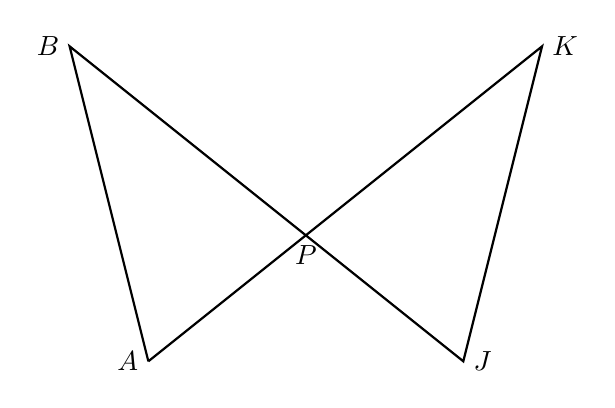
\begin{tikzpicture}
         \draw [thick]
           (-2,-1)node[left]{$A$}--
           (3,3)node[right]{$K$}--
           (2,-1)node[right]{$J$}--
           (0,0.6)node[below]{$P$}--
           (-3,3)node[left]{$B$}--(-2,-1);
       \end{tikzpicture}

     \begin{multicols}{2}
       \underline{Statement} \\
       \underline{Reason}
     \end{multicols}
     \begin{multicols}{2}
       \raggedcolumns
       \begin{enumerate}[label={\arabic*)}]
         \item $\triangle ABC$, $\triangle JKP$
         \item \rule{4cm}{0.15mm}%$\angle A \cong \angle J$ and $\overline{AP} \cong \overline{JP}$ %\vspace{0.4cm}
         \item $\angle APB \cong \angle JPK$ %
 
         \item $\triangle ABP \cong \triangle JKP$
       \end{enumerate}
       \begin{enumerate}[label={\arabic*)}]
         \item Given
         \item Given
         \item \rule{4cm}{0.15mm}
         \item \rule{4cm}{0.15mm}
       \end{enumerate}
     \end{multicols}

\newpage
\item List of theorem/situations for $\triangle \cong$ proofs
    \begin{enumerate}
      \item Vertical angles w segment bisectors
      \item Transversal corresponding
      \item Transversal with shared side on transversal
      \item Two inscribed in circle with vertical angles
      \item Inscribed in circle triangle with external angle, showing arc measure relationship
      \item Rotate triangle
      \end{enumerate}

\end{enumerate}
\end{document}